\documentclass[11pt]{article}
\usepackage[final]{acl}
\usepackage{times}
\usepackage{latexsym}
\usepackage[T1]{fontenc}
\usepackage[utf8]{inputenc}
\usepackage{microtype}
\usepackage{inconsolata}
\usepackage{graphicx}
\usepackage{booktabs}
\usepackage{amsmath}
\usepackage{amssymb}

\newcommand{\dact}{\textsc{Dact}}

\title{Knowing Where to Look Is Not Knowing What Is Right:\\
A Difference-Aware Transformer for Physical Commonsense QA}

\author{Group 69}

\begin{document}
\maketitle

\begin{abstract}
PIQA asks which of two near-identical solutions achieves an everyday physical goal. We design \dact{}, a Difference-Aware Contrastive Transformer trained from scratch, which marks the tokens where the two solutions differ, compares the solutions with cross-solution attention, pools with difference-guided attention and adds a jointly trained lexical head. With 1.9\,M parameters and no external data, \dact{} reaches 61.1\% validation and 61.6\% test accuracy (3 seeds), the best of our from-scratch models and above a TF-IDF baseline on both splits, although the test gap to that baseline is not significant. Controlled ablations show that difference tags, the lexical head and the pairwise objective each contribute, and attention controls show that the focus on differing tokens is learned rather than built in. The model finds the decisive words but cannot judge them: a fine-tuned RoBERTa is 6.3 points and a zero-shot 1.5\,B LLM 13.5 points better. We report the development history, including the failures that shaped the final design.
\end{abstract}

\section{Introduction}
Physical commonsense, knowing that \emph{baby wipes} rather than \emph{index cards} remove chalk dust, is easy for people and hard for machines. PIQA \citep{bisk2020piqa} tests it with a goal and two candidate solutions, exactly one of which is physically sensible. The task matters for assistants that give practical instructions and for robots that must choose feasible actions. Its key difficulty is that the two solutions are usually near-duplicates: in our training split the median share of differing solution tokens is 15\%, so the answer hinges on a few substituted words whose plausibility requires world knowledge.

Our aim was a model that is trained from scratch but built around this structure. \dact{} (Section~\ref{sec:method}) makes the difference between the solutions explicit at every stage: in the input, in the comparison and in the summary vector, and it adds a lexical head that scores which words make a solution plausible. We compare it with five baselines, from majority vote to a zero-shot LLM, run eight ablations with three seeds each, and analyse the attention with controls and probes.

Our main findings are: (i) \dact{} is the best from-scratch model and at least as good as a strong lexical baseline; (ii) its attention concentrates on the differing words, and controls show this focus is learned; (iii) errors come from \emph{judging} those words without physical knowledge, which only pretraining supplies. Section~\ref{sec:history} documents what worked and what did not during development.

\section{Methodology}\label{sec:method}
\begin{figure*}[t]
\centering
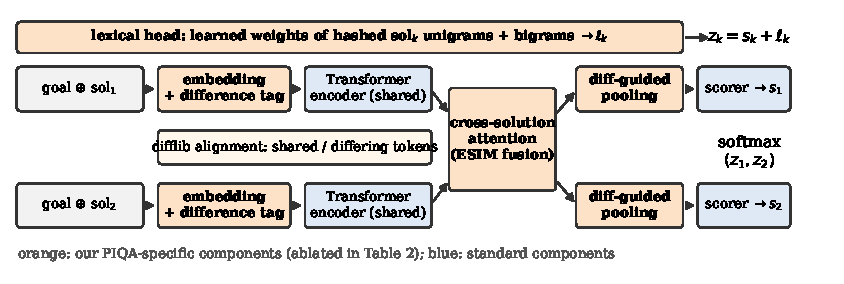
\includegraphics[width=0.97\textwidth]{figures/architecture.pdf}
\caption{\dact{}. Both options pass through the same weights, so the model is permutation-equivariant (swapping the options swaps the scores; verified in the notebook).}
\label{fig:arch}
\end{figure*}

\paragraph{Input and difference tags.} For a goal $g$ and solutions $s_1, s_2$, each option $k$ is encoded as $x^{(k)} = [\textsc{cls}]\,g\,[\textsc{sep}]\,s_k\,[\textsc{sep}]$ with a BPE vocabulary \citep{sennrich2016bpe} learned on the training split. We align the token sequences of $s_1$ and $s_2$ with \texttt{difflib} and give every solution token a tag $t_i \in \{\textit{shared}, \textit{different}\}$ (goal and special tokens: \textit{other}). The input embedding is
\begin{equation}
e_i = E_{tok}[x_i] + E_{pos}[i] + E_{seg}[\sigma_i] + E_{tag}[t_i].
\end{equation}
The tag embedding (our contribution) tells the encoder from the first layer where the options disagree.

\paragraph{Encoder.} A shared pre-LayerNorm Transformer encoder \citep{vaswani2017attention,xiong2020layer} maps each option to hidden states $H^{(k)} \in \mathbb{R}^{L \times d}$.

\paragraph{Contrastive cross-solution attention.} Each token of option $k$ attends to the solution tokens of the rival option $\bar{k}$ plus its \textsc{cls} token as a ``no counterpart'' sink:
\begin{equation}
c_i = \mathrm{MHA}\big(h^{(k)}_i, H^{(\bar{k})}, H^{(\bar{k})}\big),
\end{equation}
and the states are updated with the comparison features of ESIM \citep{chen2017esim}:
$\tilde{h}_i = \mathrm{LN}\big(h_i + \mathrm{FFN}([h_i; c_i; h_i - c_i; h_i \odot c_i])\big)$.
Adapting ESIM's local inference from premise--hypothesis pairs to two competing answers is our design choice: plausibility is relative, so each option is represented by what it has \emph{instead of} its rival.

\paragraph{Difference-guided pooling.} Over the solution tokens we use additive attention \citep{bahdanau2015neural} with a learned bias per tag (our extension):
\begin{equation}
\alpha_i \propto \exp\big(v^\top \tanh(W \tilde{h}_i) + b_{t_i}\big),\quad p = \textstyle\sum_i \alpha_i \tilde{h}_i,
\end{equation}
with $b_{\textit{different}}$ initialised to 1 and the others to 0. A scorer MLP maps $[p; \tilde{h}_{\textsc{cls}}]$ to a scalar $s_k$.

\paragraph{Lexical head.} Following the wide \& deep idea \citep{cheng2016wide}, a sparse linear component scores the words of each solution directly: every BPE unigram and bigram of $s_k$ is hashed into one of $2^{18}$ buckets with learned weight $w_j$ (initialised to 0),
\begin{equation}
\ell_k = \textstyle\sum_{j \in \mathrm{ngrams}(s_k)} w_{h(j)},\qquad z_k = s_k + \ell_k.
\end{equation}
It is trained jointly with the Transformer, with its own learning rate and weight decay. Under the pairwise softmax only $\ell_1 - \ell_2$ matters, so shared n-grams cancel and the head learns which substituted words indicate a plausible solution, the signal that a TF-IDF baseline exploits.

\paragraph{Objective.} The two scores compete in a softmax, $P(k) = \mathrm{softmax}(z_1, z_2)_k$, trained with cross-entropy and label smoothing 0.1, which matches the forced-choice task. Every component can be switched off in a single configuration object, which is how the ablations are run.

\section{Experimental Setup}
\paragraph{Data.} PIQA provides 16{,}113 training items and 1{,}838 labelled development items; the latter serve as our test set and are used only in the final evaluation. We hold out a stratified 10\% of the training file (seed 42) for validation: 14{,}501 / 1{,}612 / 1{,}838 items, all label-balanced (50.0 / 50.0 / 50.5\% label 1). Text is whitespace-normalised, NFKC-normalised and lower-cased. Goals are truncated to 40 and solutions to 96 BPE tokens; for longer solutions (1.6\% of test solutions) we keep the 96-token window centred on the differing span, not the prefix (Section~\ref{sec:history}).

\paragraph{Training.} AdamW \citep{loshchilov2019decoupled} ($\beta_2{=}0.98$, weight decay 0.05, learning rate $3{\times}10^{-4}$; lexical head $10^{-2}$), 6\% linear warm-up then cosine decay, batch 128, gradient clipping 1.0, dropout 0.2, at most 20 epochs with early stopping on validation accuracy (patience 6), fp16 mixed precision on a Colab T4. Step 1 of the notebook selects the configuration on validation with one seed from five candidates: base ($d{=}256$, 4 layers) 61.2\%, \textbf{small ($d{=}128$, 2 layers, 4 heads) 61.4\%}, base with dropout 0.3 60.8\%, and base/small with a 10-epoch in-domain masked-LM warm-up \citep{devlin2019bert} 60.8 / 60.9\%. The selected model has 1.93\,M parameters, 262\,k of them in the lexical head. The lexical head's learning rate was chosen in a separate validation pilot (Section~\ref{sec:history}).

\paragraph{Baselines.} All baseline numbers come from our own runs. \textbf{B0} majority class. \textbf{B1} TF-IDF of 1--2-grams of $s_2 - s_1$ with logistic regression, $C$ tuned on validation; it tests how far shallow lexical cues go \citep{gururangan2018annotation}. \textbf{B2} a 2-layer BiLSTM with additive attention and the same tokenizer (5.1\,M parameters), a recurrent model of similar budget. \textbf{B3} \texttt{roberta-base} \citep{liu2019roberta} fine-tuned with a multiple-choice head (4 epochs, learning rate $2{\times}10^{-5}$, 3 seeds, best epoch on validation), representing pretrained encoders. \textbf{B4} \texttt{Qwen2.5-1.5B} \citep{qwen2025qwen25} zero-shot: the prompt ``Goal: $g$ / Solution:'' followed by each solution, choosing the higher length-normalised log-likelihood, which measures LLM knowledge without any training.

\paragraph{Metrics.} Accuracy is PIQA's official metric; labels are balanced and each item has exactly one correct option, so it is unbiased with 50\% chance level. Trained models are run with seeds 42--44 and reported as mean $\pm$ std. For the seed with the best \emph{validation} accuracy we give a 95\% bootstrap CI (2{,}000 resamples; \citealp{efron1993bootstrap}) and an exact McNemar test \citep{mcnemar1947note} against \dact{} on the test set.

\section{Results and Analysis}
\begin{table}[t]
\centering\small
\begin{tabular}{@{}lcc@{}}
\toprule
Model & Val & Test \\
\midrule
\multicolumn{3}{@{}l}{\emph{trained from scratch}} \\
B0 majority & 50.0 & 50.5 \\
B1 TF-IDF + LR & 59.2 & 61.2 \\
B2 BiLSTM + attention & 59.8\,$\pm$\,0.3 & 58.7\,$\pm$\,0.9 \\
\textbf{\dact{} (ours)} & \textbf{61.1\,$\pm$\,0.8} & \textbf{61.6\,$\pm$\,0.7} \\
\midrule
\multicolumn{3}{@{}l}{\emph{pretrained}} \\
B3 RoBERTa-base, fine-tuned & 69.0\,$\pm$\,0.5 & 67.9\,$\pm$\,0.8 \\
B4 Qwen2.5-1.5B, zero-shot & 78.2 & 75.1 \\
\bottomrule
\end{tabular}
\caption{Accuracy (\%), mean $\pm$ std over 3 seeds; B0, B1 and B4 are deterministic single runs. \dact{} test 95\% CI: 59.2--63.6.}
\label{tab:main}
\end{table}

\paragraph{Overall comparison.} \dact{} is the best from-scratch model on both splits (Table~\ref{tab:main}): +1.3 / +2.9 points over the BiLSTM (McNemar $p{=}0.021$ on test) and +1.9 / +0.4 over TF-IDF. The test gap to TF-IDF is small and not significant ($p{=}0.88$), so our claim is that \dact{} is at least as good as the lexical baseline, not that it clearly beats it. Pretraining dominates: RoBERTa is 6.3 and the zero-shot LLM 13.5 points above \dact{} on test, in line with PIQA being designed to test knowledge rather than reading skill \citep{bisk2020piqa}.

\begin{table}[t]
\centering\small
\begin{tabular}{@{}lrr@{}}
\toprule
Ablation (vs.\ full \dact{}) & $\Delta$ Val & $\Delta$ Test \\
\midrule
$-$ difference tags & $-$1.4 & $-$1.3 \\
$-$ lexical head & $-$1.9 & $-$0.9 \\
pointwise (independent BCE) objective & $-$1.0 & $-$0.8 \\
mean instead of attention pooling & $-$0.2 & $-$0.9 \\
$-$ cross-solution attention & $-$0.1 & $-$0.7 \\
$-$ tag bias in pooling & +0.3 & 0.0 \\
tag bias initialised at 0 & +0.3 & 0.0 \\
\midrule
vanilla (all of the above removed) & $-$2.4 & $-$3.0 \\
\bottomrule
\end{tabular}
\caption{Ablations, 3 seeds each, one change at a time on the selected configuration; mean accuracy differences in points (seed std $\approx$ 0.3--0.9).}
\label{tab:abl}
\end{table}

\paragraph{Ablations.} Each ablation tests one hypothesis about a design choice (Table~\ref{tab:abl}); everything else, including seeds, data and budget, is fixed. \emph{Marking the difference helps}: removing the tags costs 1.4 / 1.3 points. \emph{Direct lexical evidence helps}: removing the lexical head costs 1.9 / 0.9. \emph{The forced-choice objective helps}: independent binary scoring costs 1.0 / 0.8. Removing everything costs 2.4 / 3.0 points, the largest drop. Cross-solution attention and attention pooling make no difference on validation and small ones on test, and the tag bias, including its initial value, makes none: these components overlap with the tags, which already tell the model where the options differ. Differences below one seed std are not conclusive, and with seven comparisons single p-values should not be over-read \citep{dror2018hitchhiker}.

\paragraph{Complementary errors.} \dact{} and TF-IDF agree on 78.8\% of test items; each solves about 10.6\% the other misses (197 items only \dact{}), for an oracle accuracy of 71.9\%. The items only \dact{} solves typically have a one-word difference inside long shared text (\emph{water} vs.\ \emph{soda}; the typo \emph{sparrow bottle} vs.\ \emph{spray bottle}), where a bag-of-words difference vector has almost nothing to work with. Against RoBERTa the oracle rises to 83.0\%.

\begin{figure}[t]
\centering
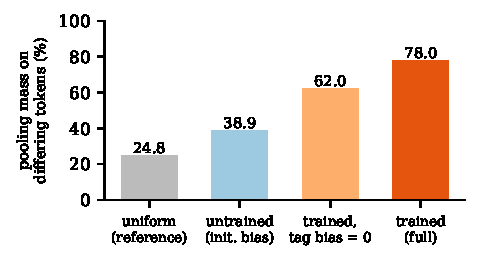
\includegraphics[width=0.92\columnwidth]{figures/attention_controls.pdf}
\caption{Share of pooling attention on differing tokens (test set). Removing the tag bias from the trained model keeps most of the focus, so it is learned, not built in.}
\label{fig:controls}
\end{figure}

\paragraph{Is the attention focus learned?} The trained model puts 84.9\% of its pooling attention on differing tokens, which make up 24.8\% of solution tokens (Figure~\ref{fig:controls}). Because the tag bias starts at 1, we separate the sources: an untrained model reaches only 38.9\%, while the trained model with the bias set to 0 still reaches 73.2\%, and the bias itself barely moved in training (1.0\,$\to$\,1.022). The focus is therefore learned by the pooling scorer, which also explains why initialising the bias at 0 changes nothing. Attention weights are not a complete explanation of a decision \citep{jain2019attention,wiegreffe2019attention}, so we use them as evidence of where the model looks, not of why it decides.

\paragraph{Why does the neural part alone not beat bag-of-words?} We tested two explanations on validation. \emph{H1: the pooling does not select} is rejected: the normalised pooling entropy is 0.51 (1 = uniform), for correct and wrong predictions alike ($p{=}0.12$). \emph{H2: the difference signal is missing}: a linear probe separating differing from shared tokens reaches 59.6\% balanced accuracy on the vanilla Transformer's embeddings and only 60.4\% after its encoder, so without tags the encoder barely works out where the options differ, whereas in \dact{} the tag remains perfectly decodable (100\%) in every layer. Tags and the lexical head thus supply information the encoder does not learn from 14.5\,k items. Crucially, wrong predictions put \emph{more} attention on the differing tokens than correct ones (86.7 vs.\ 83.8\%, $p{<}0.001$): looking at the right words is not the bottleneck; judging them is.

\begin{figure*}[t]
\centering
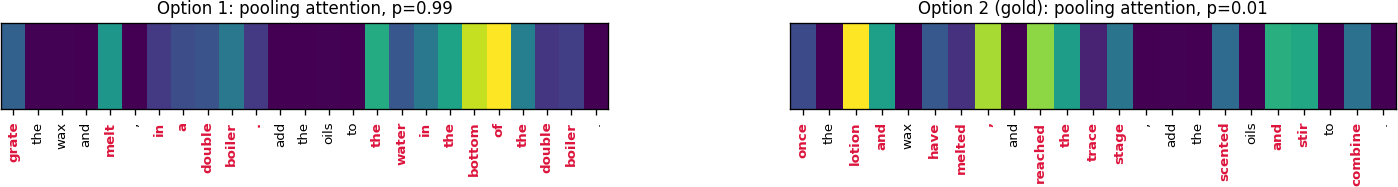
\includegraphics[width=0.98\textwidth]{figures/case_747_pooling.png}\\[3pt]
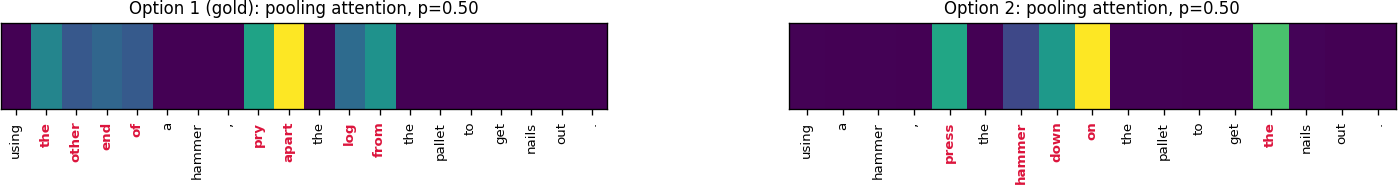
\includegraphics[width=0.98\textwidth]{figures/case_1258_pooling.png}
\caption{Pooling attention (bright = high; red = differing tokens). Top: \emph{adding scents to lotion bars}, a confident error (p = 0.99 for option 1). Bottom: \emph{how to pry pallet apart}, the most uncertain item (p = 0.50; option 1 is gold).}
\label{fig:cases}
\end{figure*}

\paragraph{Qualitative analysis.} For the item \emph{adding scents to lotion bars} (Figure~\ref{fig:cases}, top), the wrong option adds the oils ``to the water in the bottom of the double boiler''. The pooling peaks exactly on \emph{the water in the bottom}, the part that makes the option wrong, yet the model prefers it with p = 0.99: it locates the decisive span but cannot know that oil in the water bath never reaches the lotion. In \emph{how to pry pallet apart} (bottom), pooling selects the decisive spans \emph{pry apart} / \emph{other end of} vs.\ \emph{press} / \emph{hammer down on}, but the scores tie although the gold option repeats the goal words \emph{pry} and \emph{apart}: \dact{} has no explicit goal--solution matching term. Successes rest on the same word-level evidence: for \emph{a simple camping lantern}, the gold option (a milk jug on top of an \emph{LED light}, \emph{translucent plastic}) wins with p = 1.00 against \emph{fairy lights} in a filled jug, with pooling spread over the many differing words. In an earlier run, \emph{baby wipes} vs.\ \emph{index cards} for chalk dust was solved confidently; the training split contains \emph{baby wipe(s)} only in the correct option 26 times and only in the wrong option 5 times, so the confidence comes from word statistics, not from reasoning about absorbency. Finally, all four most confident predictions of the final model (p $\ge$ 0.99, right or wrong) are pairs that differ in most of their words; since $\ell_k$ is a sum over n-grams, long dissimilar options receive extreme scores, a calibration side effect of the lexical head.

\section{What Worked and What Did Not}\label{sec:history}
The final model is the result of three complete runs (and two aborted ones); all are logged in the repository, and only the last one is used in Tables~\ref{tab:main}--\ref{tab:abl}.

\paragraph{Run 1 (A100; no lexical head, prefix truncation).} \dact{} scored 60.4\% on test, \emph{below} TF-IDF (61.2\%), most single-component ablations scored higher than the full model on test, and the reported ``64\% attention on differing tokens'' could have been an artefact of the bias initialisation. One item had its only difference at BPE positions 97--98, past the 96-token limit, so both inputs were identical after truncation (p = 0.50 exactly).

\paragraph{Fixes that worked.} Difference-aware truncation keeps the differing span; in a unit check on long synthetic items it removed every case of identical inputs, and the affected PIQA item is no longer among the most uncertain predictions. The attention controls of Figure~\ref{fig:controls} turned the initialisation worry into a testable question, and the answer was that the focus is learned. Running RoBERTa with three seeds exposed its instability: in run 2 one seed stayed at chance (53.7\% validation, loss $\approx 0.694$ for all epochs), a known fine-tuning failure \citep{dodge2020finetuning}, while in the final run all seeds trained (68.4--69.4\%).

\paragraph{Engineering failures.} On the free T4, PyTorch reported bf16 as supported although it is only emulated; training ran at 377\,ms per step instead of 108\,ms with fp16, and two free-tier sessions were reclaimed after 35--40 minutes. Using bf16 only with native support and keeping a browser tab attached to the session solved both.

\paragraph{Closing the gap to bag-of-words.} Run 2 (T4, no lexical head) confirmed the picture of run 1: \dact{} 59.4 / 60.2\% vs.\ TF-IDF 59.2 / 61.2\% (val / test). We then added the lexical head. Its first version, trained with the Transformer's learning rate, did not help in a validation pilot (59.4\,$\to$\,59.5\%) because its weights barely left zero before early stopping; a separate learning rate did (3e-3: 60.5, \textbf{1e-2: 60.9}, 3e-2: 60.6\%; 3 seeds, test split not loaded). The final run confirmed the gain (61.1 / 61.6\%). \emph{Protocol note:} the head's configuration was selected on validation only, but the decision to explore a lexical component was taken after we had seen the test results of runs 1 and 2. We therefore treat the small test gap to TF-IDF as indicative rather than as a clean held-out result.

\paragraph{Evidence.} The submitted notebook contains the complete execution of the final code (commit \texttt{538cf5b}, 57 cells, no errors) with the training logs of all 30 runs; \texttt{outputs/} holds 40 JSON-lines logs, the result tables and figures; a final notebook cell asserts that tables, result files and logs agree; and \texttt{docs/DEVELOPMENT\_LOG.md} records every step, including the failed attempts above.

\section{Conclusion}
\dact{} shows that task-specific structure pays off even when training from scratch: making the difference between two near-identical solutions explicit and adding direct lexical evidence yield the best from-scratch model, and every major component is supported by a controlled ablation. Its attention demonstrably learns to focus on the decisive words. The analysis equally shows the limit of this approach: the model finds \emph{where} the options differ but judges \emph{which} is right with word statistics from 14.5\,k items, leaving it 6--14 points behind pretrained models.

\paragraph{Limitations.} Improvements of about one point are within seed and test-sample noise; hyper-parameters were selected with one seed; the lexical head is over-confident on dissimilar options; and the test comparison with TF-IDF is not fully clean (Section~\ref{sec:history}). Natural next steps are an explicit goal--solution matching term, length-normalised lexical scores, and combining the difference-aware design with pretrained representations.

\section*{Team Contributions}
\emph{[To be completed by the group: each member's contribution to design, implementation, experiments, analysis and writing.]}

\paragraph{Use of AI tools.} An AI coding assistant (Claude Code) was used extensively in this project, including for implementation, experiments and drafting this report; the full record is in \texttt{docs/DEVELOPMENT\_LOG.md}. \emph{[The group should confirm and complete this statement according to the unit's policy on AI use.]}

\bibliography{references}

\end{document}
